\documentclass[9pt]{beamer}

\usetheme{Warsaw}
\usepackage{default}
\usepackage{algorithm,algorithmic}
\usepackage{graphicx}
\usepackage{verbatim}
\usepackage{caption}
\usepackage{hyperref}
\usepackage{pgf}
\usepackage{tikz}
\usetikzlibrary{arrows,automata}
\usefonttheme{professionalfonts} % using non standard fonts for beamer
\usefonttheme{serif} % default family is serif
\usepackage{fontspec}
\setmainfont{CMU Serif}
\setmonofont{Ubuntu Mono}

\definecolor{links}{HTML}{2A1B81}
\hypersetup{colorlinks,
	linkcolor=blue,
	citecolor=pink
}

\let\oldcite=\cite
\renewcommand\cite[1]{\hypersetup{linkcolor=magenta} \hyperlink{#1}{\oldcite{#1}}}

\title{Subsequence and similarity search in biological sequences}
\subtitle{An N-Gram Graph based approach}
\author[Vasileios Charisopoulos]{Vasileios Charisopoulos}

\bibliographystyle{apalike}
\AtBeginSubsection[]
{
	\begin{frame}{Table of Contents}
		\tableofcontents[currentsubsection]
	\end{frame}
}

\begin{document}

\begin{frame}
	\titlepage
\end{frame}

\begin{frame}
\frametitle{Outline}
\tableofcontents
\end{frame}

\section{Introduction}
\begin{frame}{Motivation \& Challenges}
	\begin{itemize}
		\item<1-> Initially, focused on a more general task: graph indexing for a special class of graphs called \textit{N-Gram Graphs}
		\item<2-> Used to obtain a graph representation of text/sequential data (more about them in a few slides)
		\item<3-> Turns out this task is pretty hard - as we'll see later, the fact that some of these graphs may be similar does not let us make any strong assumptions about their sources
	\end{itemize}
	\begin{block}<4->{Queries on nucleotide databases}
	{
			Given a \textbf{database} $D$ containing nucleotide sequences and a \textbf{query sequence} $s_q$, find all entries $s_i \in D$ that contain $s_q$ (or a sequence very similar to $s_q$)
	}
	\end{block}
\end{frame}

\section{Preliminaries}
\subsection{N-Gram Graphs}
\begin{frame}{Preliminaries}
	\begin{block}<1->{What is a N-Gram Graph?}
		\begin{itemize}
			\item<1-> Introduced by George Giannakopoulos
			\item<2-> Encodes sequential data (e.g. text) into a set of \textbf{n-grams}. Every distinct n-gram becomes a vertex.
			\item<3-> $N$-gram pairs that exist within a certain distance ($D_w$) of one another are drawn as edges connecting the vertices corresponding to the co-occuring n-grams.
			\item<4-> Weight of edge connecting $n_1, n_2$ is usually the number of times $n_2$ occurs before $n_1$ within a distance $D_w$ in the text
			\item<5-> If more than a single $N$ are specified, create one such graph for each $N$ value
			\item<6->The resulting graph is called an \textit{N-Gram Graph}.
		\end{itemize}

	\end{block}
\end{frame}
\begin{frame}{Preliminaries}
	\framesubtitle{Some examples}
\begin{figure}[h]
	\centering
	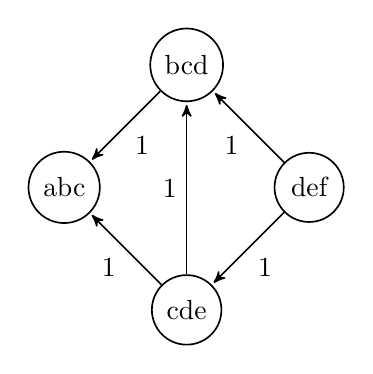
\begin{tikzpicture}[->,>=stealth',shorten >=1pt,auto,node distance=2.2cm,
	semithick]
	\tikzstyle{every state}=[fill=white,draw,text=black]
	
	\node[state] (A)                    {abc};
	\node[state] (B) [above right of=A] {bcd};
	\node[state] (C) [below right of=A] {cde};
	\node[state] (D) [below right of=B] {def};
	
	\path (B) edge node {$1$} (A);
	\path (C) edge node {$1$} (B);
	\path (C) edge node {$1$} (A);
	\path (D) edge node {$1$} (C);
	\path (D) edge node {$1$} (B);
	\end{tikzpicture}
	\caption{N-Gram Graph for ``abcdef'', $N = 3, D_w = 2$}
\end{figure}
\end{frame}
\begin{frame}{Preliminaries}
		\framesubtitle{Some examples}
What about multiple occurences of n-grams?
\begin{figure}[h]
	\centering
	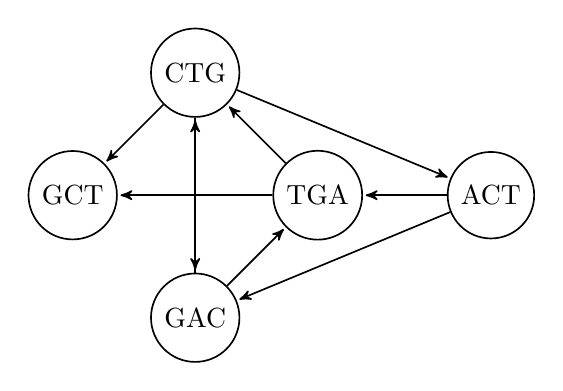
\begin{tikzpicture}[->,>=stealth',shorten >=1pt,auto,node distance=2.2cm,
	semithick]
	\tikzstyle{every state}=[fill=white,draw,text=black]
	
	\node[state] (GCT)                    {GCT};
	\node[state] (CTG) [above right of=GCT] {CTG};
	\node[state] (TGA) [below right of=CTG] {TGA};
	\node[state] (GAC) [below right of=GCT] {GAC};
	\node[state] (ACT) [right of=TGA] {ACT};	
	
	\path (CTG) edge (GCT);
	\path (CTG) edge (GAC);
	\path (CTG) edge (ACT);
	\path (TGA) edge (GCT);
	\path (TGA) edge (CTG);
	\path (GAC) edge (CTG);
	\path (GAC) edge (TGA);	
	\path (ACT) edge (TGA);	
	\path (ACT) edge (GAC);	
	\end{tikzpicture}
	\caption{N-Gram Graph for ``GCTGACTG'', $N = 3, D_w = 2$}
\end{figure}
\end{frame}

\begin{frame}{N-Gram Graph Similarity}
	In \cite{ggiannathesis}, a standard way to measure similarity is defined:
	\begin{block}{Value Similarity $\text{VS}(G_i, G_j)$}
		Equal to the sum of the value ratios, 
		$\frac{\min (w_e^i, w_e^j)}{\max (w_e^i, w_e^j)}$ for all edges that exist in both graphs, over the size of the largest of the two graphs ($ \to $ measure based on edge weight distribution).
	\end{block}
	Summarization systems with higher VS scores performed better than other existing systems (Giannakopoulos et. al).
\end{frame}

\subsection{Uses of N-Gram Graphs}
\begin{frame}{Preliminaries}
	\begin{block}<1->{Uses of N-Gram Graphs}
		\begin{enumerate}
			\item<1-> Powerful tool for document summarization
			\item<2-> Have also been applied for classification of biological data \cite{polychronopoulos2014analysis}
			\item<3-> Spam filters :) 
			\item<4-> Potentially useful for many machine learning tasks involving sequential or serializable data
		\end{enumerate}
	\end{block}
	\begin{block}<5->{Yet another task}
		Time-efficient indexing of biological sequences
	\end{block}
\end{frame}

\subsection{Nuisances about biosequence indexing}
\begin{frame}{Nuisances about biosequence indexing}
	\begin{block}<1->{Traditional methods}
		\begin{enumerate}
			\item Unlikely to avoid exhaustive searches (e.g. BLAST performs a linear scan)
			\item Might end up operating on whole sequences (oftentimes several kbp long)
			\item Lots of optimization involved even for marginally better performance
		\end{enumerate}
	\end{block}
	\begin{block}<2->{Our contribution}
		We attack the above issues, especially (1) and (2), by encoding sequences using N-Gram Graphs and using PATRICIA tries to find the most ``similar'' representations in computational time that is only slightly affected by database size.
	\end{block}
\end{frame}
	
\section{Our contribution}
\subsection{Outline}
\begin{frame}{Outline of our method}
	\begin{enumerate}
		\item<1-> Devise an encoding method for N-Gram Graphs so that similarity between graphs can be computed in constant time $t_c$. (\textit{Hashed vector encoding}, more in a few slides later)
		\item<2-> Serialize this encoding to utilize the performance of PATRICIA tries
		\item<3-> Split all database sequences in small, non-overlapping chunks (typically not longer than 100-200 bp).
		\item<4-> Index all chunks by encoding each chunk with its hash vector representation and inserting the serialized version of this into a PATRICIA trie.
	\end{enumerate}
	\begin{block}<2->{PATRICIA trie}
		Also known as radix tree - able to perform closest key queries in $\mathcal{O}(a(K))$ expected time, where $a(K)$ is the average number of bits of all items in the trie.\cite{morrison1968patricia}
	\end{block}
\end{frame}

\subsection{Similar Research}
\begin{frame}
	Similar research:
	\begin{enumerate}[(i)]
		\item \textit{Xia Cao, Shuai Cheng Li, and Anthony K. H. Tung - Indexing DNA sequences using q-grams (2005)} \cite{cao2005indexing} - Use the presence or absence of q-grams to construct a binary vector which is stored in a tree index $ \to $ does not use any information about neighborhood structure
		\item \textit{Rakthanmanon et. al. - Searching and Mining Trillions of Time Series Subsequences under Dynamic Time Warping}\cite{rakthanmanon2012searching} (2012 SIGKDD best paper award) - General purpose mining in very large scale $ \to $ lots of pruning, but doesn't avoid exhaustive scans
	\end{enumerate}
\end{frame}

\subsection{Hashed Vector Encoding}
\begin{frame}{Let's vectorize our graphs}
	\textbf{Outline of the idea:} use edge connections to include some info about the neighborhood structure into a vector representation.
	\begin{enumerate}[(i)]
		\item ``Hash'' vertices by the prefix of their labels, so that vertices with the same prefix hash to the same values (e.g. ``\colorbox{green}{AC}T'' - ``\colorbox{green}{AC}G'' hash to the same value) $ \to $ 16 distinct hash values.
		\item  Assign an encoding value to each ``bucket'' - the number of distinct vertices that are connected to any one of the vertices in that bucket $ \to$ value between $ [0, 4^N{-1}] $ for n-gram size $N$.
	\end{enumerate}
	For large enough $N$ (practically, $N \geq 3$), we expect that different DNA sequences of equal lengths will generally not produce the same encoding vector. \\
	If we want / need less bits per vector, we can quantize our values (resolution $\downarrow$, efficiency $\uparrow$).
\end{frame}
\begin{frame}{Example}
Let's revisit a previous graph:
\begin{figure}[h]
	\centering
	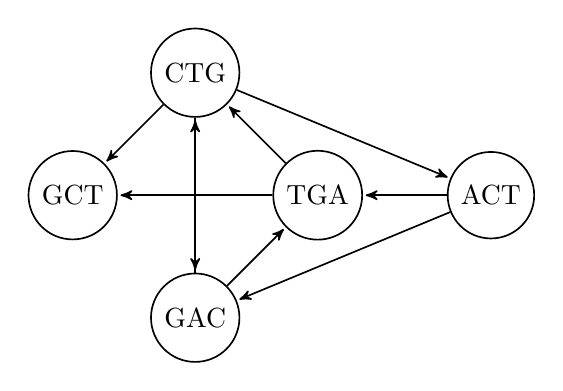
\begin{tikzpicture}[->,>=stealth',shorten >=1pt,auto,node distance=2.2cm,
	semithick]
	\tikzstyle{every state}=[fill=white,draw,text=black]
	
	\node[state] (GCT)                    {GCT};
	\node[state] (CTG) [above right of=GCT] {CTG};
	\node[state] (TGA) [below right of=CTG] {TGA};
	\node[state] (GAC) [below right of=GCT] {GAC};
	\node[state] (ACT) [right of=TGA] {ACT};	
	
	\path (CTG) edge (GCT);
	\path (CTG) edge (GAC);
	\path (CTG) edge (ACT);
	\path (TGA) edge (GCT);
	\path (TGA) edge (CTG);
	\path (GAC) edge (CTG);
	\path (GAC) edge (TGA);	
	\path (ACT) edge (TGA);	
	\path (ACT) edge (GAC);	
	\end{tikzpicture}
	\caption{N-Gram Graph for ``GCTGACTG'', $N = 3, D_w = 2$}
\end{figure}
\end{frame}
\begin{frame}{Example}
	\begin{itemize}
		\item<1-> 5 distinct prefixes: $\{ \text{GC, CT, TG, GA, AC} \} $
		\item<1-> Hash function $h$ (essentially lexicographic ordering on dinucleotides):
		\[
			h([c_1c_2c_3]) = \begin{cases}
				0 & [c_1c_2] = \text{AA} \\
				1 & [c_1c_2] = \text{AC} \\
				& \dots \\
				15 & [c_1c_2] = \text{TT}
			\end{cases}
		\]
		\item<2-> Every ``bucket'' (set of vertices that hash to the same value) has 2 incoming connections from distinct vertices, except for ``ACT''.
		\item<2-> Encoding value: 
		\[ v(G_1) = \{ 0, 1, 0, 0, 0, 0, 0, 2, 2, 2, 0, 0, 0, 0, 2, 0 \}  \]
	\end{itemize}
\end{frame}
\begin{frame}{Example}
	Now, change the graph slightly:
	\begin{figure}[h]
		\centering
		\begin{tikzpicture}[->,>=stealth',shorten >=1pt,auto,node distance=2.2cm,
		semithick]
		\tikzstyle{every state}=[fill=white,draw,text=black]
		
		\node[state] (GAT)                    {GAT};
		\node[state] (ATG) [above right of=GAT] {ATG};
		\node[state] (TGA) [below right of=ATG] {TGA};
		\node[state] (GAC) [below right of=GCT] {GAC};
		\node[state] (ACT) [right of=TGA] {ACT};	
		\node[state] (CTG) [below right of=ACT] {CTG};		
		
		\path (ATG) edge (GAT);
		\path (TGA) edge (GAT);
		\path (TGA) edge (ATG);
		\path (GAC) edge (ATG);
		\path (GAC) edge (TGA);	
		\path (ACT) edge (TGA);	
		\path (ACT) edge (GAC);	
		\path (CTG) edge (GAC);
		\path (CTG) edge (ACT);
		\end{tikzpicture}
		\caption{N-Gram Graph for ``GATGACTG'', $N = 3, D_w = 2$}
	\end{figure}
\end{frame}
\begin{frame}{Example}
	\begin{itemize}
		\item<1-> 5 distinct prefixes: $\{ \text{GA, AT, TG, AC, CT} \} $
		\item<1-> Hash function $h$ same as before
		\item<2-> The $\text{GA}$ ``bucket'' has incoming connections from:
		\[ \{ \text{ATG, TGA, ACT, CTG}  \}  \]
		\item<2-> Encoding value:
		\[ v(G_2) = \{ 0, 1, 0, 2, 0, 0, 0, 0, 4, 0, 0, 0, 0, 0, 2, 0 \}  \]
	\end{itemize}
	\begin{block}<4->{Observation}
		2 very similar sequences result in a different graph \\
		Manhattan distance:
		\[ ||\mathbf{d}||_1 = |v(G_1) - v(G_2)| = 8   \]
	\end{block}
\end{frame}
\subsection{Indexing method}
\begin{frame}{The Big Picture}
	\framesubtitle{Index construction}
	\begin{block}{In a nutshell}
		1. Pick parameters:
		\begin{itemize}
			\item Hash function $h$ and n-gram size $N$
			\item Length of indexed subsequences $L_S$
		\end{itemize}
		2. For all sequences $s$ in database $D$:
		\begin{itemize}
			\item Split $s$ into non-overlapping subsequences of length $L_S$
			\item Create an index entry containing the hashed vector encoding of each subsequence, obtain its string representation, and store it in a PATRICIA Trie.
		\end{itemize}
	\end{block}
	Assuming a fixed-size string representation of length $K$ in bits and average database sequence length $M$, the above incurs a computational cost of
	\[
		\mathcal{O}\left( \frac{|D|M}{L_S} \cdot K \right)
	\]
	
\end{frame}
\begin{frame}{The Big Picture}
	\framesubtitle{Query processing}
	Now, assume a query sequence $s_q$ is checked against the database to find matching entries:
	\begin{block}{Query Processing}
		\begin{enumerate} 
		\item<1-> Split $s_q$ in $|s_q| - L_S - 1$ subsequences of length $L_S$ with $L_S - 1$ overlap. 
		\item<2-> For every subsequence, select the ``nearest'' entry (or entries) in the Trie. Retain only those results whose manhattan distance from the subsequence falls below a threshold $T$.
		\item<3-> Stop searching after $L_S$ steps if a matching subsequence with $||\mathbf{d}||_1 = 0$ was found.
		\end{enumerate}
	\end{block}
	\uncover<3->{\textbf{Claim:} If the original sequence is part of the database (i.e. contains no mutations), a matching subsequence with $||\mathbf{d}|| = 0$ will be found after $\mathcal{O}(L_S)$ steps.}
\end{frame}
\begin{frame}{The Big Picture}
	\centering
	\includegraphics[scale = 0.5]{dna_query.eps}
\end{frame}
\begin{frame}{Remarks}
	\begin{block}{Time complexity of queries}
		\begin{enumerate}	
		\item If a query sequence is part of some database sequence, the expected time complexity of a query is 
		\[ \mathcal{O}(L_S \cdot K \cdot c(D)) \]
		\item If a query sequence $s_q$ does not appear in any of the database sequences, the expected time of a query is
		\[ 
			t_q \sim (|s_q| - L_S - 1) \cdot K \cdot c(D)
		\]
		$L_S$: size of indexed subsequences \\
		$K$: the length (in bits) of the encoding vectors' string representation \\
		$c(D)$: collision factor $ \to $ the average number of entries in the constructed index that have the same encoding vector
	\end{enumerate}
	\end{block}
\end{frame}
\begin{frame}{Remarks}
	\begin{block}{Advantages \& Limitations}
		\begin{itemize}
			\item<1-> Query sequences $s_q$ must have length $|s_q| \geq 2 \cdot L_S$. If $|s_q| << L_S$, no proper alignment is possible. 
			\item<2-> Distance used is not edit distance - however, we know that two identical sequences produce exactly the same encoding vector.
			\item<3-> Computing that distance can be done in $\mathcal{O}(4^{L})$, where $L < N$. Value Similarity required $\mathcal{O}(E) = \mathcal{O}(4^{2N})$.
			\item<4-> If we can avoid large collision coefficients, query time is not affected by database size!
		\end{itemize}
	\end{block}
\end{frame}
\begin{frame}{Parameter tuning}
	\begin{block}{Everything is a tradeoff}
		\begin{itemize}
			\item<1-> We should avoid small prefix lengths $L$ ( typically $ L > 2 $) in order to avoid colliding entries. Larger $L$ gives us more resolution but also increases key size $K$.
			\item<2-> Using vertex degree as the encoding value, we can guarantee that it will be in $[0, 4^{N} - 1] $ for every index $\to $ fixed range for serialization.
			\item<3-> A large $L_S$ typically increases the chances that two subsequences will produce the same encoding vector, as well as the time complexity for query sequences that are not part of $D$. On the other hand, small $L_S$ add more entries to the database.
		\end{itemize}
	\end{block}
\end{frame}
\begin{frame}{Other concerns}
	\begin{block}<1->{Memory Footprint}
		In Theory: $K$ bits per encoding vector, subsequence length $L_S$. Denoting the average length (in bp) by $\overline{L}$, we need roughly
		\[ n_{\text{entries}} = \Theta(|D| \cdot \frac{\overline{L}}{L_S}) \]
		entries in the constructed trie for a total (in bits) of
		\[
		   K_{\text{total}} = \Theta(|D| \cdot K \frac{\overline{L}}{L_S})
		\]
	\end{block}
	\begin{block}<2->{The truth is always a little worse}
		In Java, a large memory overhead is incurred by the lack of ease in bit manipulation and the Patricia trie \href{https://commons.apache.org/proper/commons-collections/apidocs/org/apache/commons/collections4/trie/PatriciaTrie.html}{implementation}.
	\end{block}
\end{frame}
\subsection{Experiments}
\begin{frame}{Experiments}
	In the following experiments, we set $L_S = 150, N = 3, L = 2$ (key size $K = 1024$ bits).
	\begin{columns}
		\begin{column}{0.5\textwidth}  %%<--- here
			\begin{block}{E.Coli experiment}
				\begin{itemize}
					\item Database size: $\simeq 5 MB$, contains 400 entries in FASTA format -- Number of indexed fragments: $30,875$
					\item $200$ randomly selected query sequences of length $L_q = 300$.
					\item<2->{\textbf{Results}:
						\begin{itemize}
							\item Recall: $ 200 / 200 $ 
							\item Avg. Query Time $\overline{t_q}$: $213.05$ ms
							\item Avg. Answer Set Size: $4.665$
						\end{itemize}
					}
				\end{itemize}
			\end{block}	
		\end{column}
	\begin{column}{0.5\textwidth}
		\begin{block}<3->{D. Melanogaster Experiment}
			\begin{itemize}
				\item Database size: $\simeq 119 MB$, contains 1170 entries in FASTA format -- Number of indexed fragments: $817,091$
				\item $100$ randomly selected query sequences of length $L_q = 1500$ 
				\item<4->{\textbf{Results}:
					\begin{itemize}
						\item Recall: $ 100 / 100 $
						\item Avg. Query Time $\overline{t_q}: 224.91 $ms
						\item Avg. Answer Set Size: 1.05
					\end{itemize}
				}
			\end{itemize}
		\end{block}
	\end{column}	
	\end{columns}
\end{frame}
\begin{frame}{Effect of $L_S$ on $\overline{t}_q$}
	\begin{block}{Reminder}
		$L_S$: length of indexed subsequences
	\end{block}
	Expectation: if $L_S \uparrow $, $t_q \uparrow $ because of the larger window that must be checked exhaustively.
	We repeat the D. Melanogaster experiments with $L_S = \{ 100, 300 \}$:
	\begin{columns}
		\begin{column}{0.5 \textwidth}
			\begin{block}<2->{$L_S = 100$}
				\begin{itemize}
					\item Number of indexed fragments: $1,255,968$
					\item \textbf{Results:}
					\begin{itemize}
						\item Recall: $ 100 / 100 $
						\item Avg. Query Time $\overline{t}_q: 122.87 $ms
						\item Avg. Answer Set Size: 1.03
					\end{itemize}
				\end{itemize}
			\end{block}
		\end{column}
		\begin{column}{0.5 \textwidth}
			\begin{block}<3->{$L_S = 300$}
				\begin{itemize}
					\item Number of indexed fragments: $408,249$
					\item \textbf{Results:}
					\begin{itemize}
						\item Recall: $ 100 / 100 $
						\item Avg. Query Time $\overline{t}_q: 649.97 $ms
						\item Avg. Answer Set Size: 1.03
					\end{itemize}
				\end{itemize}
			\end{block}
		\end{column}
	\end{columns}
\end{frame}
\begin{frame}{Experimental Validation}
	\begin{itemize}
	\item Despite the fact that $|D|_{\text{melanogaster}} \geq 20 \cdot |D|_{\text{ecoli}}$, the average query times for the same $L_S$ only differ by roughly $5 \% \to $ query time only slightly affected by $|D|$!
	\item On the other hand, increasing $L_S$ had a clear effect on execution time. In the case where $L_S = 300$, the query time is almost 3 times as large as when $L_S = 150 \to $ suggests using a small $L_S$.
	\end{itemize}
	\begin{block}<2->{Pending improvement}
		Solving the memory overhead problem is our greatest concern.
	\end{block}
\end{frame}
\begin{frame}{More fine-tuning}
	Noticing that the average answer set size is considerably small for both cases, we gave a shot at fine tuning by further reducing $L_S$ and $K$: 
	\begin{columns}
	\begin{column}{0.5 \textwidth}
		\centering
		\includegraphics[width = \textwidth]{query_perf.eps}
	\end{column}
	\begin{column}{0.5 \textwidth}
		\centering
		\begin{tabular}{r | c c c}
			$L_S$ & Recall & $\overline{t}_q$(ms) & $\#$Matches \\ \hline
			$ 20 $  & $100\%$ & 3.04 & 9.07 \\
			$ 30 $  & $100\%$ & 9.45 & 1.53 \\
			$ 40 $  & $100\%$ & 12.45 & 1.09 \\
			$ 50 $  & $100\%$ & 17.40 & 1.05 \\
			$ 60 $  & $100\%$ & 28.54 & 1.04 \\
			$ 70 $  & $100\%$ & 34.52 & 1.06 \\
			$ 80 $  & $100\%$ & 48.71 & 1.06
		\end{tabular}
	\end{column}
	\end{columns}
	Running the BLAST algorithm (\texttt{ncbi-blast+} package in Debian) for the same query gave a performance of $\overline{t}_q \simeq 18$(ms).
\end{frame}
\section{Future Directions}
\begin{frame}{Pending improvements}
	\begin{block}<1->{Implementation}
		\begin{enumerate}[(i)]
			\item The current \texttt{PatriciaTrie} implementation incurs a heavy overhead on memory because it only allows \texttt{String} keys $ \to $ 2 bytes per digit as per the Java Standard.
			\item Our implementation only works with databases that are fully loaded in RAM so far.
			\item Potential for parallelization; could solve the above issue in a distributed computing model.
		\end{enumerate}
	\end{block}
	\begin{block}<2->{Research}
		\begin{enumerate}[(i)]
			\item More work (i.e. experiments \& verification) needed on how to choose $N, h, L_S$ etc.
			\item Need to test on larger datasets ( $ \geq 1 GB $) to measure scaling potential after solving the memory overhead issue.
		\end{enumerate}
	\end{block}
\end{frame}
\section{References}
\begin{frame}[allowframebreaks]
	\frametitle{References}
	\nocite{papadakis2015graph}
	\nocite{rajaraman2012mining}
	\bibliography{demokritos_bib}
\end{frame}

\begin{frame}{Reproducible research}
	\begin{itemize}
	\item Source code is available in \texttt{Github} under the \texttt{GPLv3} license: \href{https://github.com/VHarisop/BioGraphs}{\texttt{https://github.com/VHarisop/BioGraphs}} (\texttt{git clone} us!)
	\item All of the datasets are available from the NCBI \href{ftp://ftp.ncbi.nlm.nih.gov/blast/db/}{FTP Server} (\texttt{ecoli.nt, drosoph.nt}).
	\item The query sequences were generated using \texttt{query\_generator.py} from the \texttt{scripts/tools/} directory of \texttt{BioGraphs}.
	\end{itemize}
\bigskip\textbf{Thanks to}: George Giannakopoulos for supervising this project :) 
\end{frame}

\begin{frame}
	\centering
	\Huge Thank you! \\Questions?
\end{frame}

\end{document}
